\documentclass[aspectratio=169]{beamer}
\usepackage{UAH-theme}
\usepackage{minted}
\usepackage{xcolor}
% Use a placeholder if you don't have the actual logo
% Create a simple UAH logo placeholder
\usepackage{tikz}
\usepackage{array}
\usepackage{multirow}
\usepackage{array}
\usepackage{colortbl}
\usepackage{booktabs}
\usepackage{graphicx} 
\usepackage[many]{tcolorbox}


\usetikzlibrary{arrows.meta, positioning}
\usetikzlibrary{shapes, arrows, positioning}
\definecolor{stackaddr}{RGB}{173,216,230}
\definecolor{stackval}{RGB}{255,228,181}
\definecolor{stackdesc}{RGB}{144,238,144}
\definecolor{addr}{RGB}{173,216,230}
\definecolor{val}{RGB}{255,228,181}
\definecolor{desc}{RGB}{144,238,144}

\newcommand{\UAHLogoPlaceholder}{%
\begin{tikzpicture}[scale=0.15]
\draw[fill=UAHred,draw=none] (0,0) circle (5);
\draw[white,line width=0.5mm] (0,0) circle (4);
\draw[white,line width=0.5mm] (-2,2) -- (2,2);
\draw[white,line width=0.5mm] (-2,-2) -- (2,-2);
\draw[white,line width=0.5mm] (0,4) -- (0,-4);
\end{tikzpicture}%
}

\definecolor{frame1}{RGB}{255, 230, 230}
\definecolor{frame2}{RGB}{230, 255, 230}
\definecolor{frame3}{RGB}{230, 230, 255}
\definecolor{frame4}{RGB}{255, 255, 230}

\definecolor{androidBlue}{HTML}{8AB4F8}
\definecolor{androidBlueLight}{HTML}{E8F0FE}
\definecolor{androidGreen}{HTML}{81C995}
\definecolor{androidGreenLight}{HTML}{E6F4EA}

% Red variants - based on Android's "error" and warning colors
\definecolor{androidRed}{HTML}{F28B82}
\definecolor{androidRedLight}{HTML}{FADAD7}

% Yellow variants - based on Android's accent/warning colors
\definecolor{androidYellow}{HTML}{FDD663}
\definecolor{androidYellowLight}{HTML}{FEF7E0}

% Purple variants - based on Android's system UI accents
\definecolor{androidPurple}{HTML}{D7AEFB}
\definecolor{androidPurpleLight}{HTML}{F4EAFC}

% Orange variants - based on Android's notification colors
\definecolor{androidOrange}{HTML}{FCAD70}
\definecolor{androidOrangeLight}{HTML}{FEEADC}

% Teal variants - based on Android's Material You palette
\definecolor{androidTeal}{HTML}{78D9EC}
\definecolor{androidTealLight}{HTML}{E6F6F9}

% Gray variants - based on Android's neutral colors
\definecolor{androidGray}{HTML}{DADCE0}
\definecolor{androidGrayLight}{HTML}{F1F3F4}



\usemintedstyle{default}
\setminted{
fontsize=\footnotesize,
frame=single,
linenos=true,
breaklines=true,
autogobble=true
}


\title{11 Floating Point Operations in ARM}
\subtitle{CPE 221}
\author{Rahul Bhadani}
\institute{The University of Alabama in Huntsville}
\date{\today}


\begin{document}

\begin{frame}

    \titlepage

\end{frame}

\begin{frame}{}
    \tableofcontents
\end{frame}

\section{Introduction to Floating-Point Support in ARMv7}
\begin{frame}
    \sectionpage
\end{frame}

\begin{frame}{ARMv7 VFP Architecture Overview}
\begin{itemize}
\item ARMv7 provides hardware floating-point support through:
\begin{itemize}
\item Vector Floating Point (VFP) extension
\item Advanced Single Instruction, Multiple Data (SIMD), NEON extension
\end{itemize}
\item CPULator supports these extensions
\item VFP supports IEEE 754 single-precision and double-precision operations
\item Key components:
\begin{itemize}
\item Dedicated register set
\item Special instructions for floating-point operations
\item Control and status register (FPSCR)
\end{itemize}
\end{itemize}
\end{frame}

\begin{frame}{Two Separate Processors}
    \begin{center}
        \includegraphics[width=1.0\textwidth]{../figures/Two_processors.pdf}
    \end{center}
\end{frame}

\section{Floating-Point Register Set}
\begin{frame}
    \sectionpage
\end{frame}

\begin{frame}{Floating-Point Register Organization}
    \begin{itemize}
    \item ARMv7 VFP provides 32 single-precision registers (S0-S31)
    \item These can be viewed as:
    \begin{itemize}
    \item 16 double-precision registers (D0-D15)
    \item S0/S1 overlap with D0, S2/S3 with D1, etc.
    \end{itemize}
    \item Advanced implementations support 32 double-precision registers (D0-D31)
    \item VFP/NEON registers are separate from general-purpose registers
    \end{itemize}
    \begin{center}
    \begin{tabular}{|c|c|c|c|}
    \hline
    \textbf{Single-precision} & S0 & S1 & ... \\ % Fixed: Added "\\" to end the row
    \hline
    \textbf{Double-precision} & \multicolumn{2}{|c|}{D0} & ... \\ % Fixed: Added "\\" to end the row
    \hline
    \end{tabular}
    \end{center}
\end{frame}

\begin{frame}{FPSCR: Floating-Point Status and Control Register}
    \begin{itemize}
    \item Special register that controls VFP operation
    \item Contains fields for:
    \begin{itemize}
    \item Exception flags (N, Z, C, V)
    \item Rounding mode configuration
    \item Exception handling controls
    \item Vector length/stride control
    \end{itemize}
    \item Similar role to the CPSR for integer operations
    \item Accessible via special instructions:
    \begin{itemize}
    \item VMRS - Move from FPSCR to ARM register
    \item VMSR - Move to FPSCR from ARM register
    \item APSR\_nzcv (Application Program Status Register, NZCV flags): The APSR holds the condition flags for integer operations. The \_nzcv suffix specifies that only the N (Negative), Z (Zero), C (Carry), and V (Overflow) flags should be updated.
    \end{itemize}
    \end{itemize}
\end{frame}



\section{Basic Floating-Point Operations}
\begin{frame}
    \sectionpage
\end{frame}

\begin{frame}[fragile]{VMOV}

    \begin{minted}{asm}
        .data
            pi_val: .float 3.14159
            double_val: .double 1.618
        
        .text
        .global _start
        _start:
            VMOV S0,0.5
        done: B done
        \end{minted}

VMOV only works with a  limited set of constants. VMOV constants are limited to $\pm m/2^{k}$. Bit 7: Sign bit. Bits 6:4: $0 \leq k \leq 7$, Bits 3:0: $16 \leq m \leq 31$

This is not supported in CPULator.

\end{frame}

\begin{frame}[fragile]{Loading and Storing Floating-Point Values}
\begin{minted}{asm}
.data
    pi_val: .float 3.14159
    double_val: .double 1.618

.text
.global _start
_start:
    LDR R0, =pi_val
    VLDR S0, [R0]        @ Load single-precision constant
    
    LDR R0, =double_val
    VLDR D1, [R0]        @ Load double-precision constant
	
done: B done
\end{minted}
Supported in CPULator.
\end{frame}

\begin{frame}[fragile]{Basic Arithmetic Operations}
    \begin{minted}{asm}
    @ Single-precision operations
    VADD.F32 S0, S1, S2         @ S0 = S1 + S2
    VSUB.F32 S3, S4, S5         @ S3 = S4 - S5
    VMUL.F32 S6, S7, S8         @ S6 = S7 * S8
    VDIV.F32 S9, S10, S11       @ S9 = S10 / S11
    @ Double-precision operations
    VADD.F64 D0, D1, D2         @ D0 = D1 + D2
    VSUB.F64 D3, D4, D5         @ D3 = D4 - D5
    VMUL.F64 D6, D7, D8         @ D6 = D7 * D8
    VDIV.F64 D9, D10, D11       @ D9 = D10 / D11
    \end{minted}
\end{frame}


\begin{frame}[fragile]{Division Operation}
\begin{minted}[linenos,frame=single,fontsize=\footnotesize]{gas}
.global _start
_start:
    // Load the floating-point numbers into registers using PC-relative addressing
    VLDR.F32 S0, float1   // Load 37.24 into register S0
    VLDR.F32 S1, float2   // Load 7.51 into register S1
    // Perform the division: S2 = S0 / S1
    VDIV.F32 S2, S0, S1   // S2 = S0 / S1
    // At this point, S2 contains the result of 37.24 / 7.51
    // Exit the program (optional, depending on your environment)
    MOV R7, #1            // syscall: exit
done: B done
    // Define the floating-point constants in a literal pool
    .ltorg                // Place the literal pool here
float1: .float 37.24
float2: .float 7.51
\end{minted}
\end{frame}

% \begin{frame}[fragile]{Entry Point Definition}
% \begin{minted}[frame=single,fontsize=\footnotesize]{gas}
% .global _start
% \end{minted}

% \begin{itemize}
% \item Makes the symbol \texttt{\_start} globally visible to the linker
% \item Marks the entry point of the program
% \item Essential for the linker to know where execution begins
% \end{itemize}
% \end{frame}

% \begin{frame}[fragile]{Program Start Label}
% \begin{minted}[frame=single,fontsize=\footnotesize]{gas}
% _start:
% \end{minted}

% \begin{itemize}
% \item Defines the \texttt{\_start} label
% \item Execution of the program begins at this point
% \item Standard entry point name for many assembly programs
% \end{itemize}
% \end{frame}

\begin{frame}[fragile]{Loading First Floating-Point Value}
\begin{minted}[frame=single,fontsize=\footnotesize]{gas}
VLDR.F32 S0, float1   // Load 37.24 into register S0
\end{minted}

\begin{itemize}
\item \texttt{VLDR.F32}: Vector Load instruction for 32-bit floating-point values
\item \texttt{S0}: Destination register (single-precision floating-point)
\item \texttt{float1}: Label referencing memory location with value 37.24
\item Uses PC-relative addressing to locate the value
\end{itemize}
\end{frame}

\begin{frame}[fragile]{Loading Second Floating-Point Value}
\begin{minted}[frame=single,fontsize=\footnotesize]{gas}
VLDR.F32 S1, float2   // Load 7.51 into register S1
\end{minted}

\begin{itemize}
\item Similar to previous instruction
\item Loads 32-bit floating-point value 7.51 from memory
\item Places value into register S1
\item Prepares second operand for division operation
\end{itemize}
\end{frame}

\begin{frame}[fragile]{Performing Floating-Point Division}
\begin{minted}[frame=single,fontsize=\footnotesize]{gas}
VDIV.F32 S2, S0, S1   // S2 = S0 / S1
\end{minted}

\begin{itemize}
\item \texttt{VDIV.F32}: Vector Floating-Point Division instruction
\item Divides value in S0 (37.24) by value in S1 (7.51)
\item Result stored in register S2
\item Calculates $37.24 \div 7.51 \approx 4.96$
\end{itemize}
\end{frame}



\begin{frame}[fragile]{Literal Pool Directive}
\begin{minted}[frame=single,fontsize=\footnotesize]{gas}
.ltorg                // Place the literal pool here
\end{minted}

\begin{itemize}
\item \texttt{.ltorg}: Directive to place a literal pool at this location
\item Literal pool: Storage area for constants not directly encodable in instructions
\item Ensures floating-point constants are accessible to VLDR instructions
\item Important for proper memory layout and addressing
\end{itemize}
\end{frame}

\begin{frame}[fragile]{Floating-Point Constant}
\begin{minted}[frame=single,fontsize=\footnotesize]{gas}
float1: .float 37.24
float2: .float 7.51
\end{minted}

\begin{itemize}
\item \texttt{float1:}: Label to reference this memory location
\item \texttt{.float 37.24}: Allocates space for 32-bit floating-point constant
\item Defines the first operand for our division operation
\item Referenced by the first VLDR instruction
\item \texttt{float2:}: Label for memory reference
\item \texttt{.float 7.51}: Allocates space for 32-bit floating-point constant
\item Defines the second operand (divisor)
\item Referenced by the second VLDR instruction
\end{itemize}
\end{frame}

\begin{frame}[fragile]{Comparison and Conditional Operations}
    \begin{minted}{asm}
    @ Compare floating-point values
    VCMP.F32 S0, S1             @ Compare S0 with S1
    VMRS APSR_nzcv, FPSCR       @ Transfer flags to APSR
    BEQ equal_label             @ Branch if S0 == S1
    BGT greater_than_label      @ Branch if S0 > S1
    
    @ Using VPSEL (ARMv8 but supported in some ARMv7 implementations)
    VCMP.F32 S0, S1
    VMRS APSR_nzcv, FPSCR
    VMOVGT.F32 S2, S0           @ Move S0 to S2 if S0 > S1
    \end{minted}
\end{frame}

\section{Data Conversion}
\begin{frame}
    \sectionpage
\end{frame}

\begin{frame}[fragile]{Converting Between Formats}
\begin{minted}{asm}
@ Integer to floating-point
VMOV S0, R0                 @ Move R0 value to S0
VCVT.F32.S32 S0, S0         @ Convert signed 32-bit int to float
@ Floating-point to integer
VCVT.S32.F32 S1, S0         @ Convert float to signed 32-bit int
VMOV R1, S1                 @ Move S1 value to R1

@ Single to double precision
VCVT.F64.F32 D0, S0         @ Convert single to double

@ Double to single precision
VCVT.F32.F64 S2, D0         @ Convert double to single
\end{minted}
\end{frame}

\section{Working with FPSCR}
\begin{frame}
    \sectionpage
\end{frame}

\begin{frame}[fragile]{Accessing FPSCR}
\begin{minted}{asm}
@ Reading FPSCR
VMRS R0, FPSCR              @ Read FPSCR into R0
@ Writing to FPSCR
VMSR FPSCR, R0              @ Write R0 to FPSCR

@ Moving flags from FPSCR to APSR
VMRS APSR_nzcv, FPSCR       @ Copy condition flags

@ Setting rounding mode (example: round to nearest)
MOV R0, #0x0                @ Round to nearest mode
BIC R1, R0, #0x00C00000     @ Clear rounding mode bits
ORR R1, R1, #0x00000000     @ Set round to nearest (00)
VMSR FPSCR, R1              @ Update FPSCR
\end{minted}
\end{frame}

\section{Loading Floating Data Memory to Multiple Registers}
\begin{frame}
    \sectionpage
\end{frame}

\begin{frame}{VLDMIA}
    \begin{columns}
        \column{0.5\linewidth}
        Load Multiple FPU  Registers, Increment After.

        \textbf{Syntax:}
    
        \texttt{VLDMIA Rn!,register list}
        \begin{itemize}
            \item FP registers $\to$ memory, 1st address in Rn
            \item Updates Rn only if write-back flag (!) is  appended to Rn.
        \end{itemize}
        Example: 

        \texttt{// Copy starting at mem[R0]}
        
        \texttt{VLDMIA R0!,\{S0,S1,S2\}}
        \column{0.5\linewidth}
        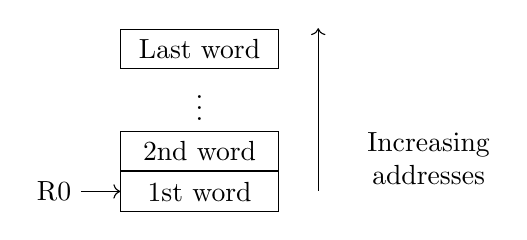
\begin{tikzpicture}
            \node (first_word) [draw, minimum width=2cm, minimum height=0.5cm, anchor=west] {1st word};
            \node (second_word) [draw, minimum width=2cm, minimum height=0.5cm, above=0cm of first_word] {2nd word};
            \node (dots) [above=0cm of second_word] {$\vdots$};
            \node (last_word) [draw, minimum width=2cm, minimum height=0.5cm, above=0cm of dots] {Last word};
            
                \node (ro) [left=0.5cm of first_word] {R0};
                \draw[->] (ro) -- (first_word.west);
            
                \coordinate (arrow_start) at ([xshift=0.5cm, yshift=0.01cm]first_word.east);
                \node (increasing_addresses) [yshift=0.41cm, right=0.5cm of arrow_start, anchor=west, align=center] {Increasing\\ addresses};
                \draw[->] (arrow_start) -- ([xshift=0.5cm, yshift=0.01cm]last_word.north east);
            \end{tikzpicture}
            
    \end{columns}
\end{frame}

\begin{frame}{VLDMDB}
    \begin{columns}
        \column{0.5\linewidth}
        Load Multiple FPU  Registers, Decrement Before.

        \textbf{Syntax:}

        
        \texttt{VLDMDB Rn!,register list}
        \begin{itemize}
            \item FP registers $\to$ memory, addresses end 
            just before address in Rn
            \item Must append  (!) and always updates Rn.            
        \end{itemize}
        Example: 

        \texttt{//Copy ending before mem[R0]}

        \texttt{VLDMDB R0!,\{S0,S1,S2\}}
        \column{0.5\linewidth}
        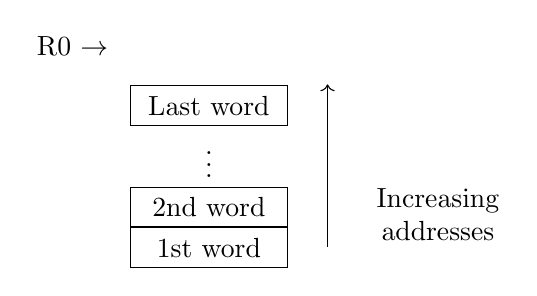
\begin{tikzpicture}
            \node (first_word) [draw, minimum width=2cm, minimum height=0.5cm, anchor=west] {1st word};
            \node (second_word) [draw, minimum width=2cm, minimum height=0.5cm, above=0cm of first_word] {2nd word};
            \node (dots) [above=0cm of second_word] {$\vdots$};
            \node (last_word) [draw, minimum width=2cm, minimum height=0.5cm, above=0cm of dots] {Last word};
            
                \node (ro) [left=0.15cm of last_word, yshift=0.75cm,] {R0 $\to$};
            
                \coordinate (arrow_start) at ([xshift=0.5cm, yshift=0.01cm]first_word.east);
                \node (increasing_addresses) [yshift=0.41cm, right=0.5cm of arrow_start, anchor=west, align=center] {Increasing\\ addresses};
                \draw[->] (arrow_start) -- ([xshift=0.5cm, yshift=0.01cm]last_word.north east);
            \end{tikzpicture}
            
    \end{columns}
\end{frame}

\section{Examples}
\begin{frame}
    \sectionpage
\end{frame}

\begin{frame}[fragile]{Example 1: Computing the Area of a Circle}
\begin{minted}[fontsize=\tiny]{asm}
    .data
    pi: .float 3.14159265       @ Single-precision PI
    radius: .float 5.0          @ Circle radius
    area: .float 0.0            @ Result storage
    .text
    .global _start
    _start:
    @ Load the radius and PI into VFP registers
    LDR R0, =radius
    VLDR S0, [R0]               @ S0 = radius
    LDR R0, =pi
    VLDR S1, [R0]               @ S1 = pi
    
    @ Compute radius squared
    VMUL.F32 S2, S0, S0         @ S2 = radius * radius
    
    @ Compute area = pi * radius^2
    VMUL.F32 S3, S1, S2         @ S3 = pi * radius^2
    
    @ Store the result
    LDR R0, =area
    VSTR S3, [R0]               @ Store result to memory
    
    done: B done
\end{minted}
\end{frame}

\begin{frame}[fragile]{Example 2: Temperature Conversion}
    \begin{minted}[fontsize=\tiny]{asm}
    .data
    temp_f: .float 98.6         @ Temperature in Fahrenheit
    temp_c: .float 0.0          @ Will hold Celsius result
    const_32: .float 32.0       @ Constant for conversion
    const_5_9: .float 0.5555555 @ 5/9 as a floating-point constant
    .text
    .global _start
    _start:
    @ Load the Fahrenheit temperature
    LDR R0, =temp_f
    VLDR S0, [R0]               @ S0 = fahrenheit temperature
    @ Load the constants
    LDR R0, =const_32
    VLDR S1, [R0]               @ S1 = 32.0
    LDR R0, =const_5_9
    VLDR S2, [R0]               @ S2 = 5/9
    @ Formula: C = (F - 32) * 5/9
    VSUB.F32 S3, S0, S1         @ S3 = F - 32
    VMUL.F32 S4, S3, S2         @ S4 = (F - 32) * 5/9
    @ Store the result
    LDR R0, =temp_c
    VSTR S4, [R0]               @ Store Celsius result
    
    done: B done
    \end{minted}
\end{frame}

\begin{frame}[fragile]{Example 3: Working with FPSCR for Exception Handling}
    \begin{columns}
        \column{0.2\linewidth}
        \column{0.8\linewidth}
        \begin{minted}[fontsize=\footnotesize]{asm}
            .data
            val1: .float 1.0
            val2: .float 0.0            @ Will cause division by zero
            .text
            .global _start
            _start:
            @ Enable floating-point exceptions (division by zero)
            VMRS R0, FPSCR              @ Read current FPSCR
            ORR R0, R0, #(1 << 2)       @ Set DZE (Division by Zero) exception bit
            VMSR FPSCR, R0              @ Update FPSCR
            @ Load values
            LDR R0, =val1
            VLDR S0, [R0]               @ S0 = 1.0
            LDR R0, =val2
            VLDR S1, [R0]               @ S1 = 0.0
        \end{minted}
    \end{columns}
    \end{frame}
    
    \begin{frame}[fragile]{Example 3: Working with FPSCR for Exception Handling (Continued)}
        \begin{columns}
            \column{0.2\linewidth}
            \column{0.8\linewidth}
            \begin{minted}[fontsize=\footnotesize]{asm}

            @ Try division that will cause exception
            VDIV.F32 S2, S0, S1         @ S2 = S0 / S1 (div by zero)
            @ Check for exception
            VMRS R0, FPSCR              @ Read FPSCR after operation
            TST R0, #(1 << 2)           @ Check if DZC (Division by Zero) flag is set
            BNE division_error          @ Branch if exception occurred
            B continue                  @ No exception, continue
            division_error:
            @ Handle the error here
            MOV R0, #1                  @ Error code
            B end
            continue:
            MOV R0, #0                  @ Success code
            end:
            done: B done
            \end{minted}
    \end{columns}

\end{frame}


\begin{frame}
    \Huge{\centerline{\color{androidGreen}\textbf{The End}}}
\end{frame}


\end{document}